% Carried over verbatim from monograph/main.tex (Study 1 record, 13 Sep 2026).
\chapter{Datasets and the hidden hierarchy}\label{s1:ch:ch04_datasets_and_the_hidden_hierarchy}

\section{Overview}

\begin{table}[H]
\centering
\caption{Audited datasets and independent units.}
\label{s1:tab:datasets}
\begin{tabularx}{\textwidth}{lrrrXX}
\toprule
Dataset & Observations & Parents & Mean/parent & Released task & Parent definition \\
\midrule
SIPaKMeD & 4,049 & 966 & 4.19 & 5-class classification & cluster field \\
Cx22 & 1,320 & 514 & 2.57 & semantic/instance segmentation & CCEDD source image \\
CRIC & 11,534 & 400 & 28.84 & cytology classification resource & source smear image \\
Herlev & 917 & 917 & 1.00 & 7-class single-cell classification & released cell image \\
\bottomrule
\end{tabularx}
\end{table}

\begin{figure}[H]
\centering
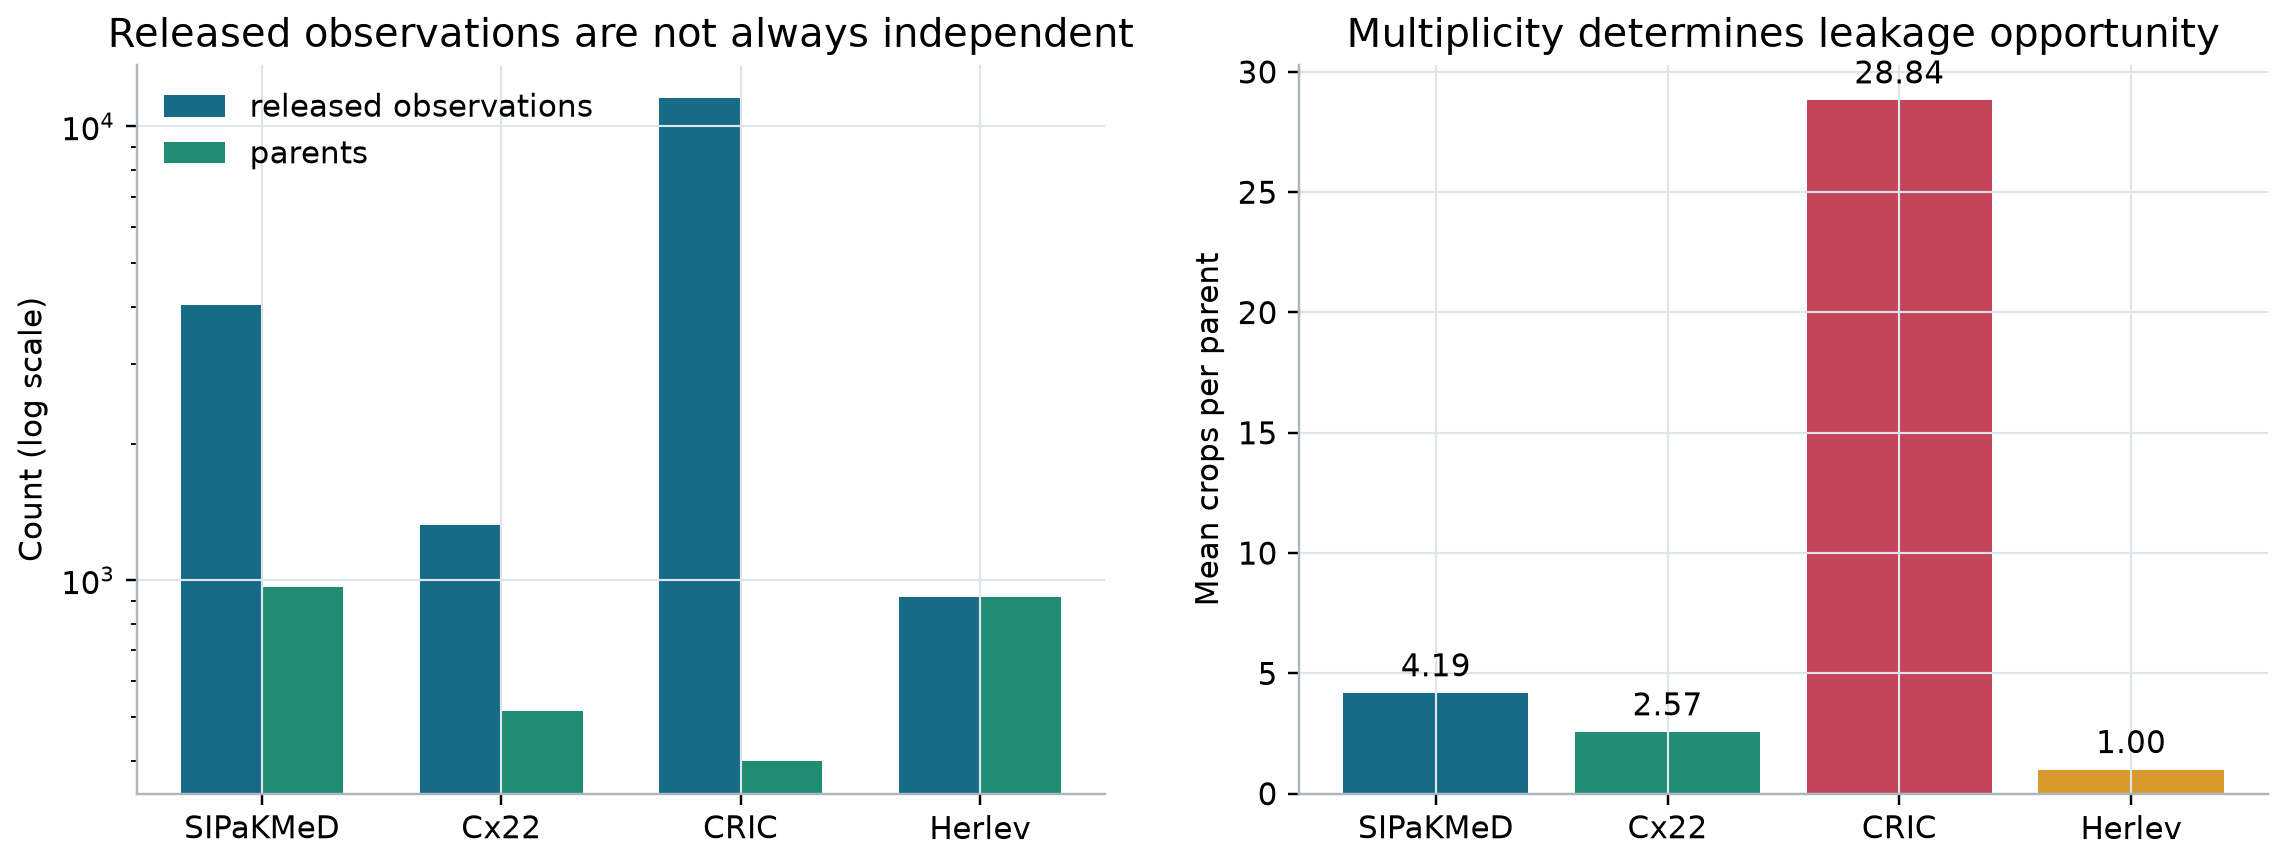
\includegraphics[width=\textwidth]{dataset_scale.png}
\caption{Dataset scale and mean parent multiplicity. The log-scale left panel prevents CRIC's 11,534 observations from visually erasing the smaller datasets.}
\label{s1:fig:dataset-scale}
\end{figure}

\begin{figure}[H]
\centering
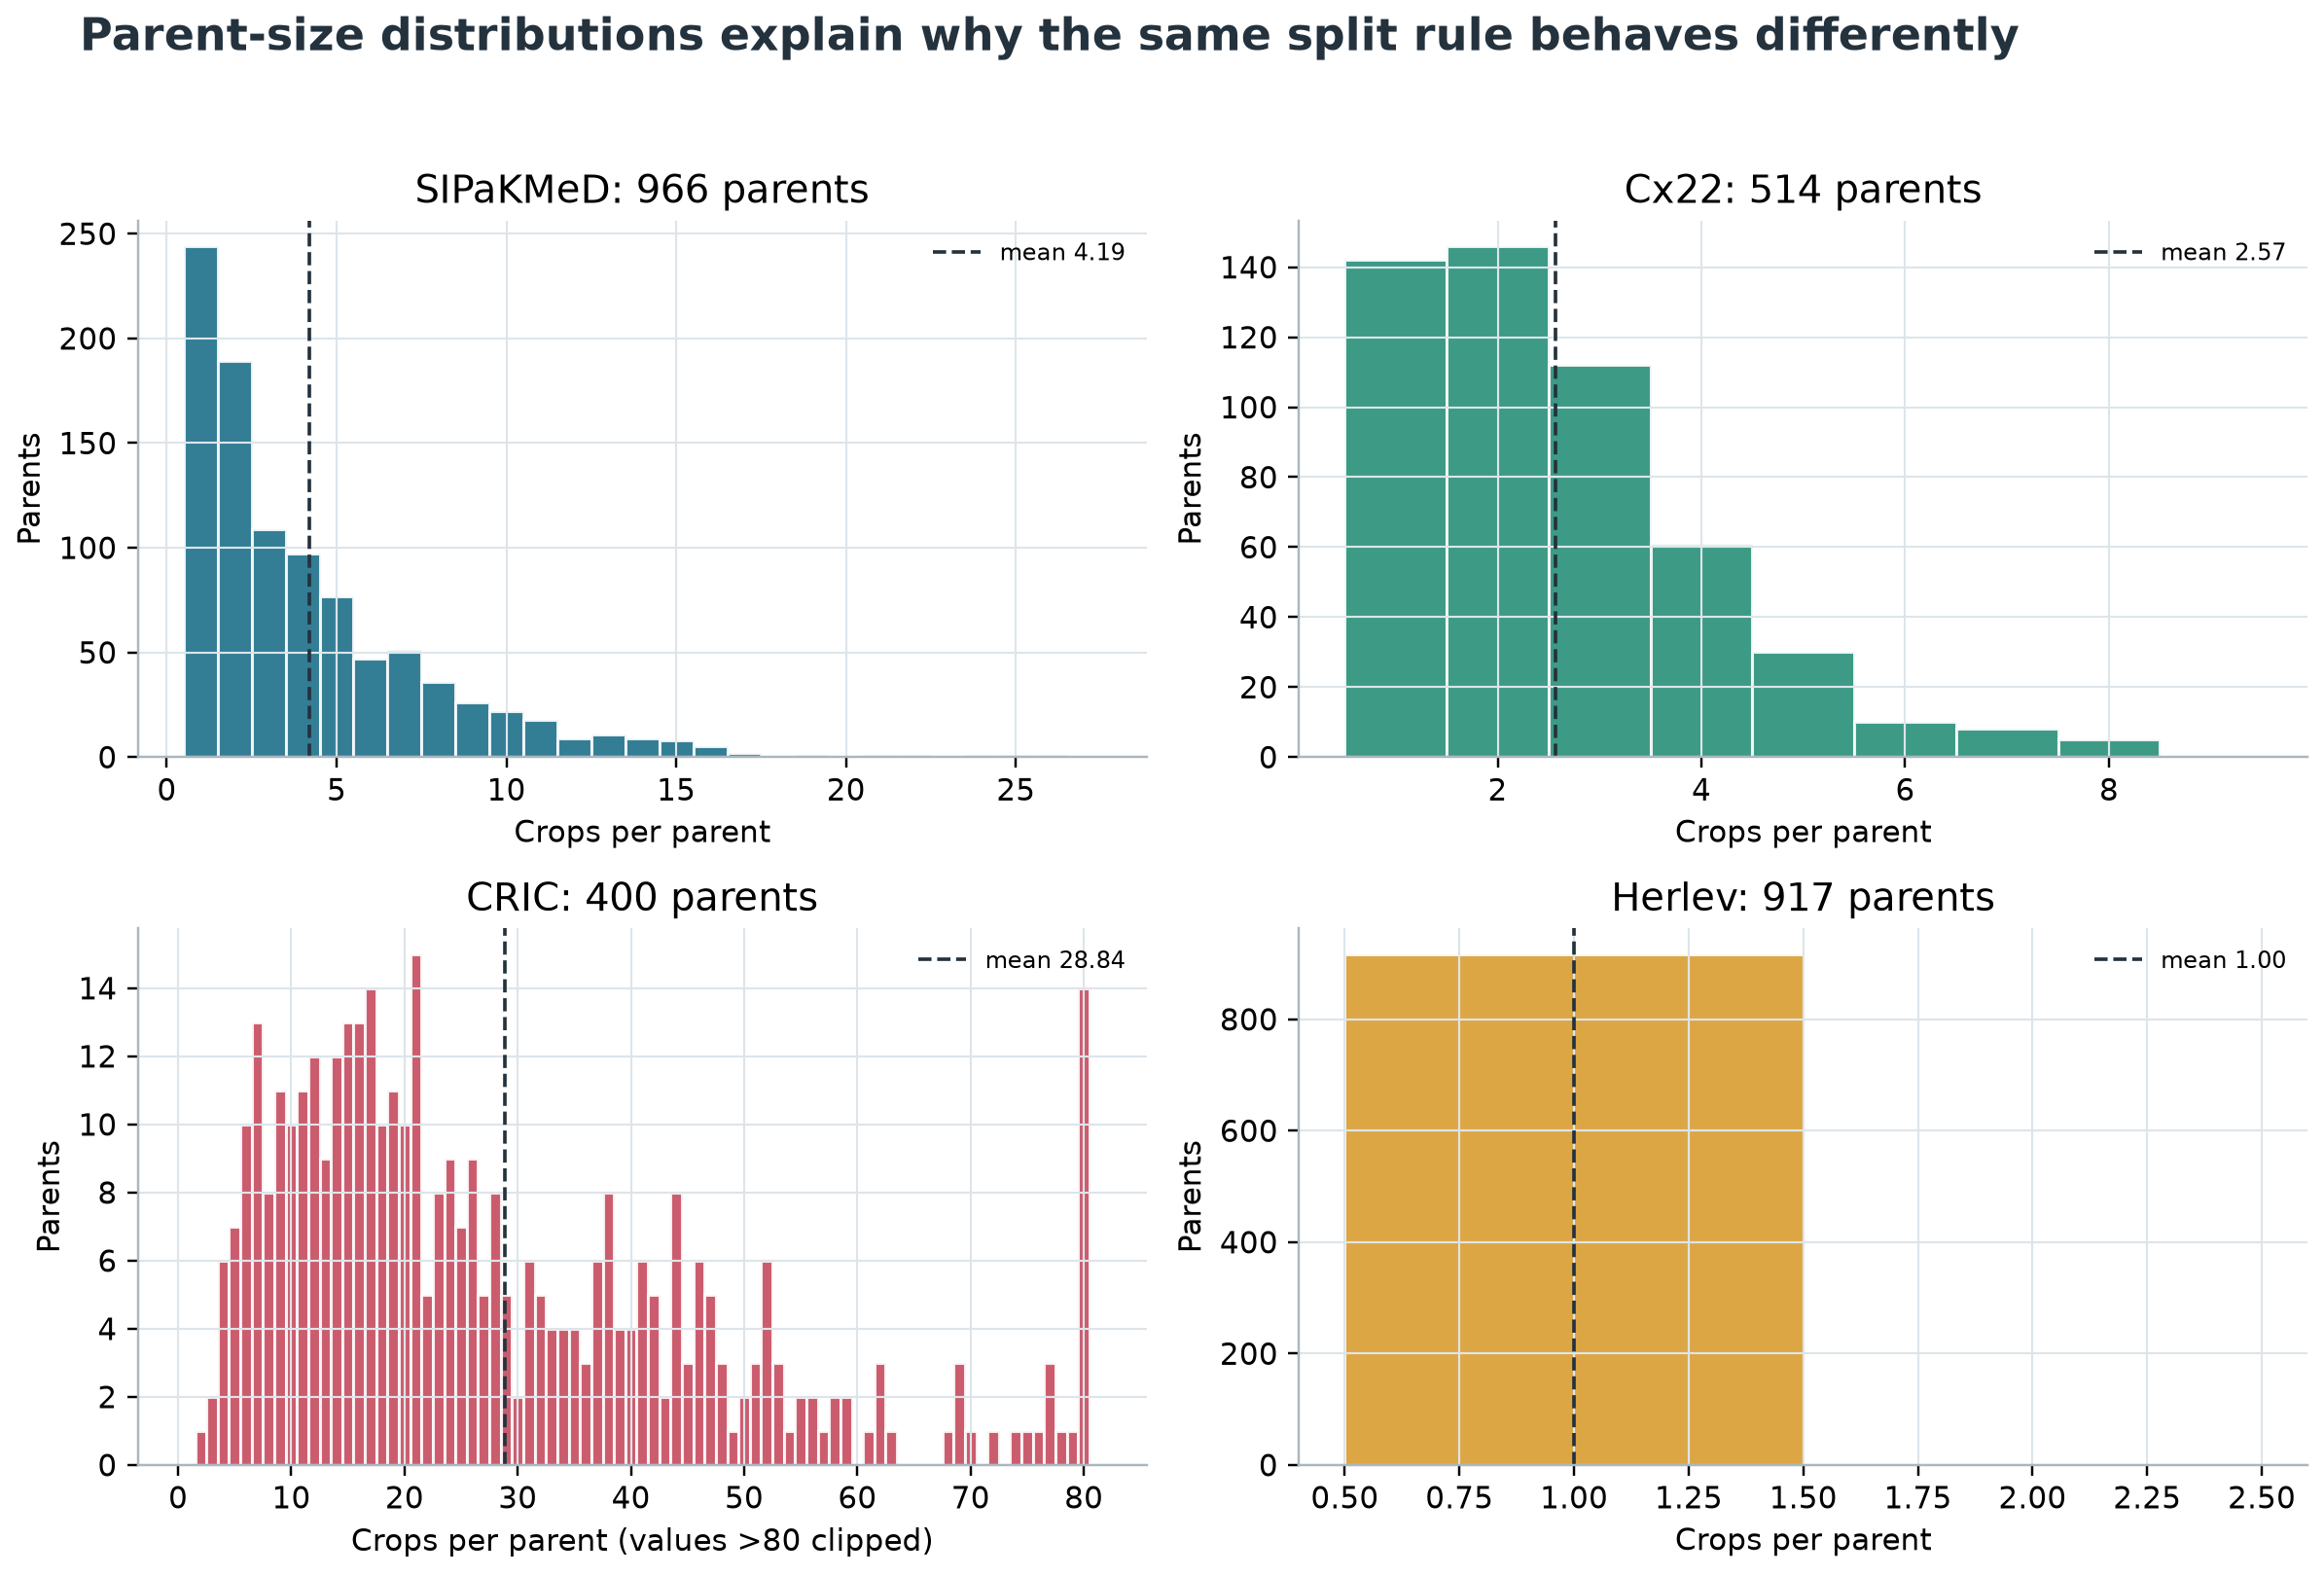
\includegraphics[width=\textwidth]{parent_size_distributions.png}
\caption{Complete parent-size distributions recovered from the Parquet maps. High multiplicity drives the probability that random crop splitting places a parent in both arms.}
\label{s1:fig:parent-distributions}
\end{figure}

\section{SIPaKMeD}

SIPaKMeD contains 4,049 isolated cell images derived from 966 cluster fields~\cite{plissiti2018sipakmed}. The released hierarchy is unusually valuable for an audit: full fields and a \artifact{CROPPED} directory coexist, and crop filenames encode the field identifier. The project uses the cluster field---not the crop file---as the parent.

\begin{table}[H]
\centering
\caption{Independently reconstructed SIPaKMeD class totals in release order.}
\label{s1:tab:sip-classes}
\begin{tabular}{lrrr}
\toprule
Class & Crops & Parents & Crops/parent \\
\midrule
Superficial--Intermediate & 831 & 126 & 6.60 \\
Parabasal & 787 & 108 & 7.29 \\
Koilocytotic & 825 & 238 & 3.47 \\
Metaplastic & 793 & 271 & 2.93 \\
Dyskeratotic & 813 & 223 & 3.65 \\
\midrule
Total & 4,049 & 966 & 4.19 \\
\bottomrule
\end{tabular}
\end{table}

The class order deserves explicit mention because the original planning text swapped the final two names even though its numerical vector was right. The integrity gate exposed that inconsistency, and Amendment 1 corrected it before results existed. This is an example of a check preventing a quiet metadata error.

\section{Cx22 and CCEDD}

Cx22 provides 1,320 generated regions and instance labels, drawing source images from CCEDD~\cite{liu2022cx22}. Three released subsets are involved: Multi-Train, Multi-Test, and Pair. The parent is the named CCEDD source image. Generator metadata provide source name and requested ROI coordinates; the authors' MATLAB generator defines how a source rectangle is clipped, resized, and pasted into a 512-by-512 white canvas.

The official Multi-Train and Multi-Test arms have zero shared parents. Pair is separately released and shares 55 parents with Multi-Test (Jaccard 0.126) and 233 with Multi-Train (Jaccard 0.475). The later model matrix pools all 1,320 observations only as a preregistered stress test of downstream reuse. It is not an accusation that the official authors used a leaking split.

\begin{figure}[H]
\centering
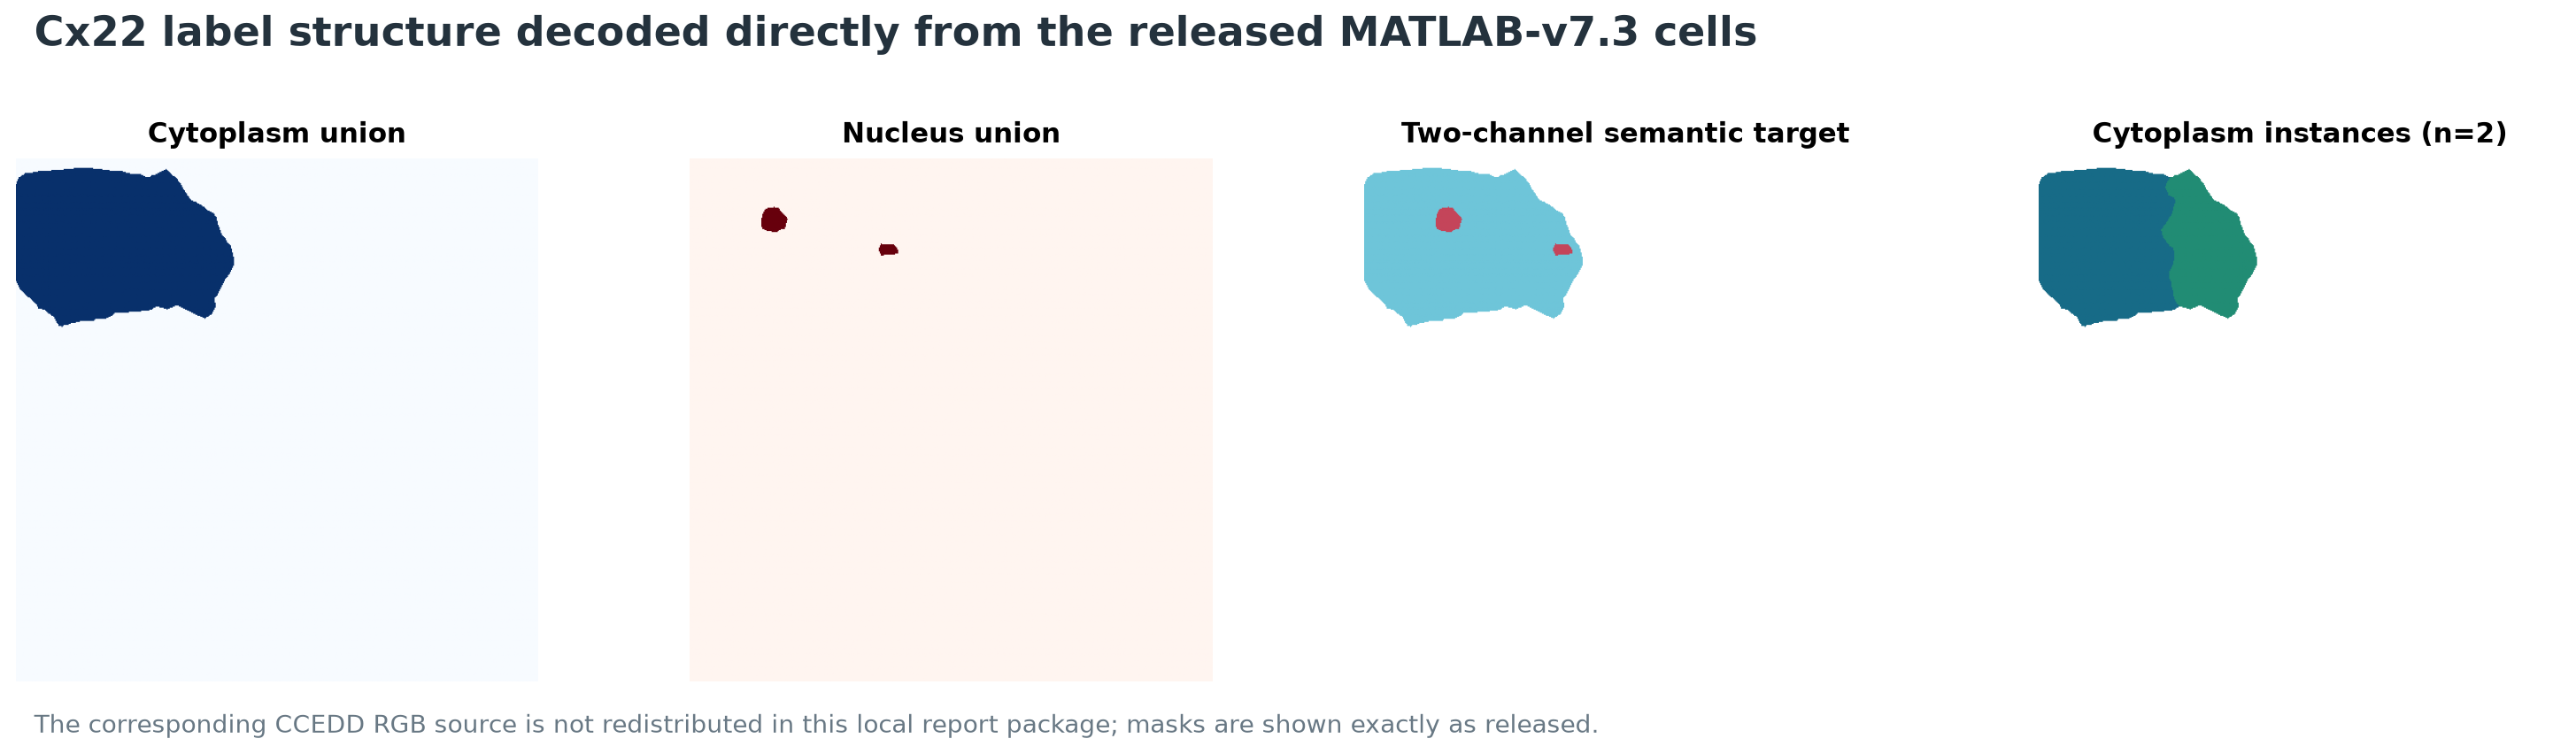
\includegraphics[width=\textwidth]{cx22_label_structure.png}
\caption{One released Cx22 Pair target decoded from the MATLAB-v7.3 structures. Cytoplasm and nucleus unions define two non-exclusive semantic channels; individual cytoplasm masks define the instance task. The CCEDD RGB source is not redistributed in this report.}
\label{s1:fig:cx22-labels}
\end{figure}

\section{CRIC}

CRIC contains 11,534 classified cells associated with 400 source images~\cite{rezende2021cric}. The released classification table supplies source identity and cell coordinates, which makes source-level grouping deterministic. A reliable patient identifier is not present in the released table, so the project does not claim patient-disjoint evaluation. This matters: source-image grouping is stronger than crop grouping but can still be weaker than patient grouping.

\section{Herlev as a structural negative control}

Herlev contains 917 released single-cell images~\cite{jantzen2005pap}. Under the project's declared data unit, each image is one observation and one parent. It therefore has no multi-observation parent structure and must return exactly zero parent straddling. If Herlev showed a nonzero structural effect, the implementation would be wrong. The control passed for all five seeds.

\section{Data-use constraints}

The repository publishes identifiers, coordinates, hashes, split assignments, code, and derived statistics. It does not redistribute raw images. Cx22/CCEDD material is restricted to non-commercial research/education in the declared source manifest, and CCEDD redistribution is prohibited. CRIC and the local Herlev repackaging are declared CC BY 4.0. SIPaKMeD's source notes require citation and experimental use. The complete URL/checksum/terms ledger appears in \cref{s1:tab:data-sources}.
